\documentclass[a4paper, 9pt]{article}
\usepackage[utf8]{inputenc}
\usepackage[T1]{fontenc}
\usepackage{xcolor}
\usepackage{parskip}
\usepackage{enumitem}
\usepackage{graphicx}

\date{\today}
\author{Diedler Baptiste}
\title{Réseaux}

\begin{document}
\maketitle
    \section{définition}
    \begin{description}[style=nextline]
        \item[communication de circuits:]
        (+) qualité de service/facturation.\\
        (-) mauvaise utilisation des ressources
    
        \item[transfert de paquets:]
        (+) meilleur utilisation des ressources, plus rapide.\\
        (-) les paquets peuvent arriver désordonnés et nécessité d'un contrôle de flux pour connaître le chemin à prendre.

        \item[communication:]
        L'adresse de destination n'intervient pas dans le processus de décision d'acheminement.

        \item[trame:]
        Paquet dont on sait reconnaître le début et la fin.

        \item[paquet:]
        Trame dont on ne sait pas reconnaître le début et la fin.
    \end{description}

    \section{classification}
        \subsection{type de transmision}
            \begin{description}[style=nextline]
                \item[réseau à diffusion:]
                Dispose d'un seul canal de transmission, qui est partagé par tous les équipements qui y sont connextés. Toutes les machines reçoivent les données et seul la destination les lit.

                \item[réseau point à point:]
                Grand nombre de connexions, chacune faisant intervenir deux machines. POur aller de la source à la destination, les données peuvent transsister par plusieurs machines.
            \end{description}

        \subsection{topologie}
            \begin{description}[style=nextline]
                \item[topologie physique:]
                Qui décrit comment les machines sont raccordées au réseau.

                \item[topologie logique:]
                Qui renseigne sur le mode d'échange des données dans le réseau.
            \end{description}

            La topologie du réseau est souvent influencée par différents facteurs:\\
            configuration du site, nombre de stations à connecter, flux des
            données, coût, distance entre entités communicantes, évolution
            possible, résistance aux pannes et lignes de secours, administration.

            \begin{description}[style=nextline]
                \item[topologie en bus:]
                Une topologie en bus est l'organisation la plus simple d'un réseau. Tous les
                ordinateurs sont reliés à une même ligne de transmission par l'intermédiaire d’un
                câble, généralement coaxial. Le mot « bus » désigne la ligne physique.
            \end{description}
            \begin{figure}[ht]
                \centering
                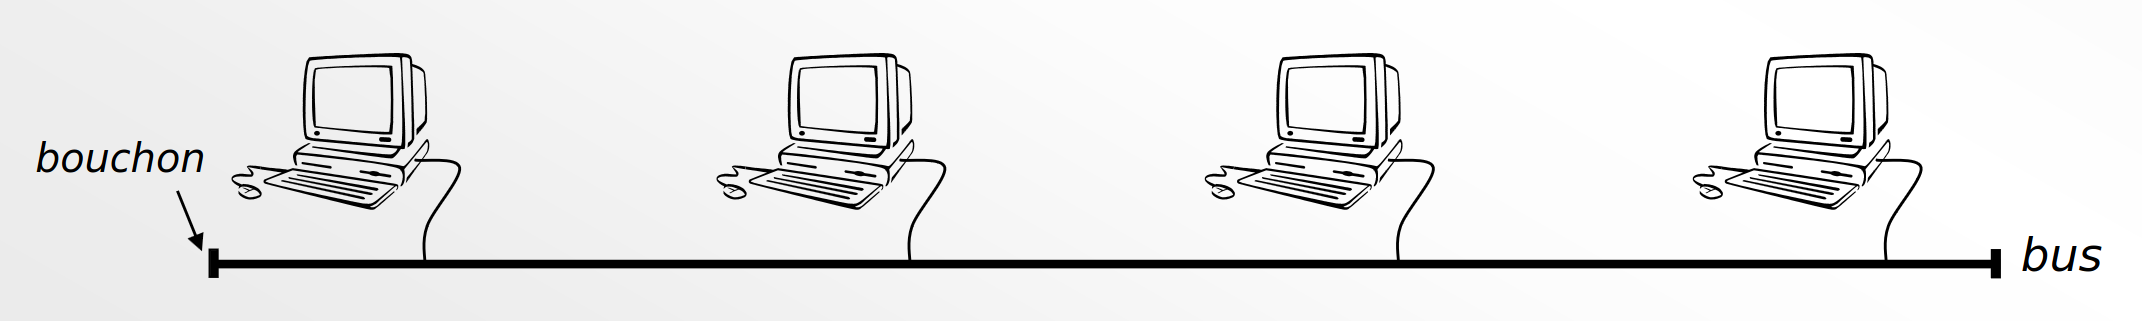
\includegraphics[width=0.8\textwidth]{topologie_bus.png}
                \caption{Topologie en bus}
                \label{fig:topologie_bus}
            \end{figure}
            \begin{description}[style=nextline]
                \item[topologie en anneau:]
                Dans la topologie en anneau, chaque poste est connecté au suivant.
                L’information circule dans un seul sens. Chaque station réémet les données et
                les recopie si elles lui sont destinées.
            \end{description}
            \begin{figure}[ht]
                \centering
                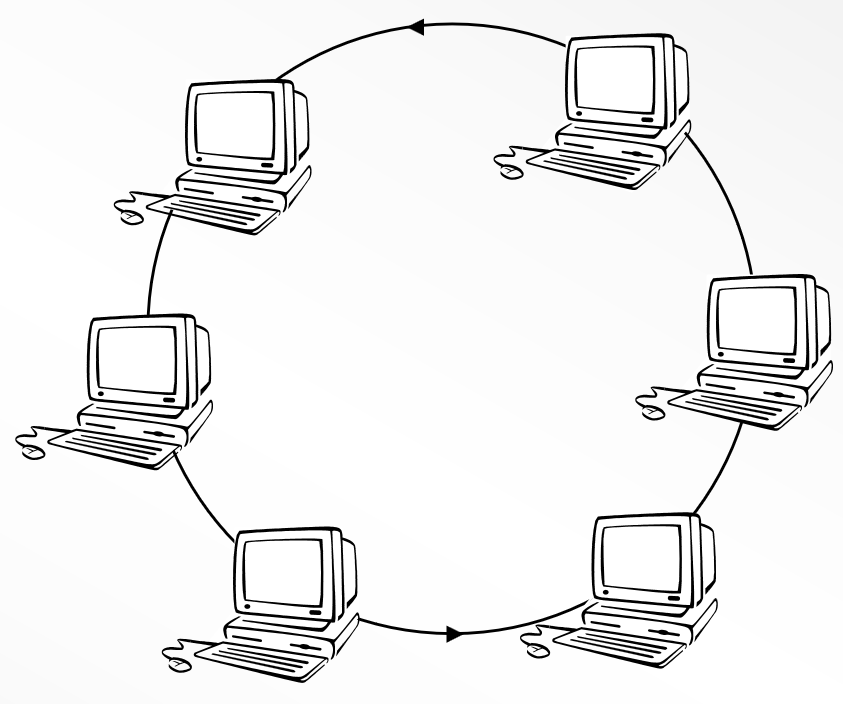
\includegraphics[width=0.3\textwidth]{topologie_anneau.png}
                \caption{Topologie en anneau}
                \label{fig:topologie_anneau}
            \end{figure}
            \begin{description}[style=nextline]
                \item[topologie en étoile:]
                La topologie en étoile est une variante de la topologie point-à-point. Un nœud
                central, appelé concentrateur (hub) émule n liaisons point-à-point. Tous les
                nœuds du réseau sont reliés au nœud central.
            \end{description}
            \begin{figure}[ht]
                \centering
                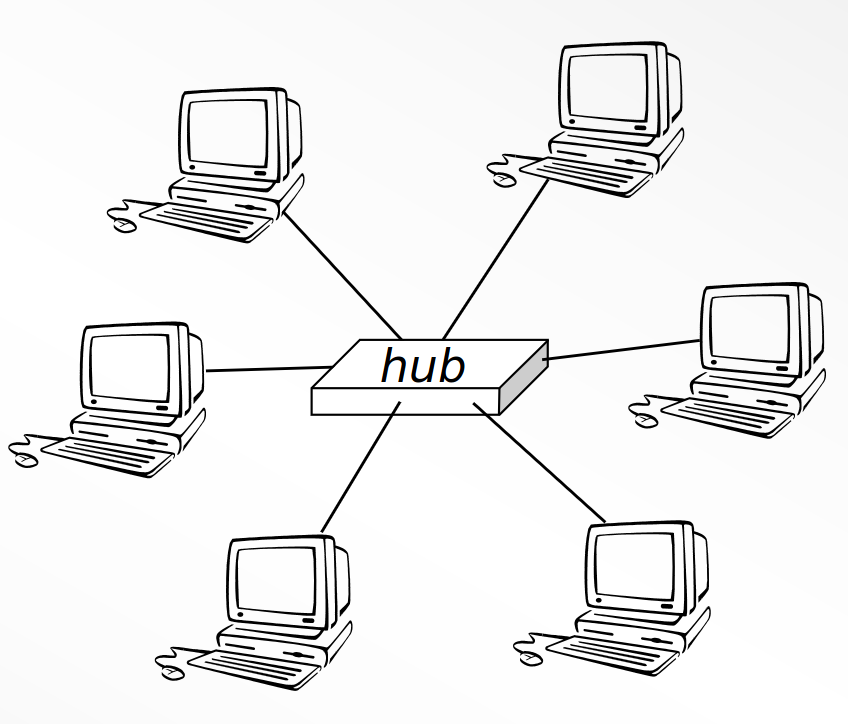
\includegraphics[width=0.3\textwidth]{topologie_etoile.png}
                \caption{Topologie en étoile}
                \label{fig:topologie_etoile}
            \end{figure}
            \begin{description}[style=nextline]
                \item[topologie en arbre:]
                Un réseau arborescent est constitué d’un ensemble de réseaux en étoile,
                reliés en par des concentrateurs jusqu’à un nœud unique (nœud de tête).
            \end{description}
            \begin{figure}[ht]
                \centering
                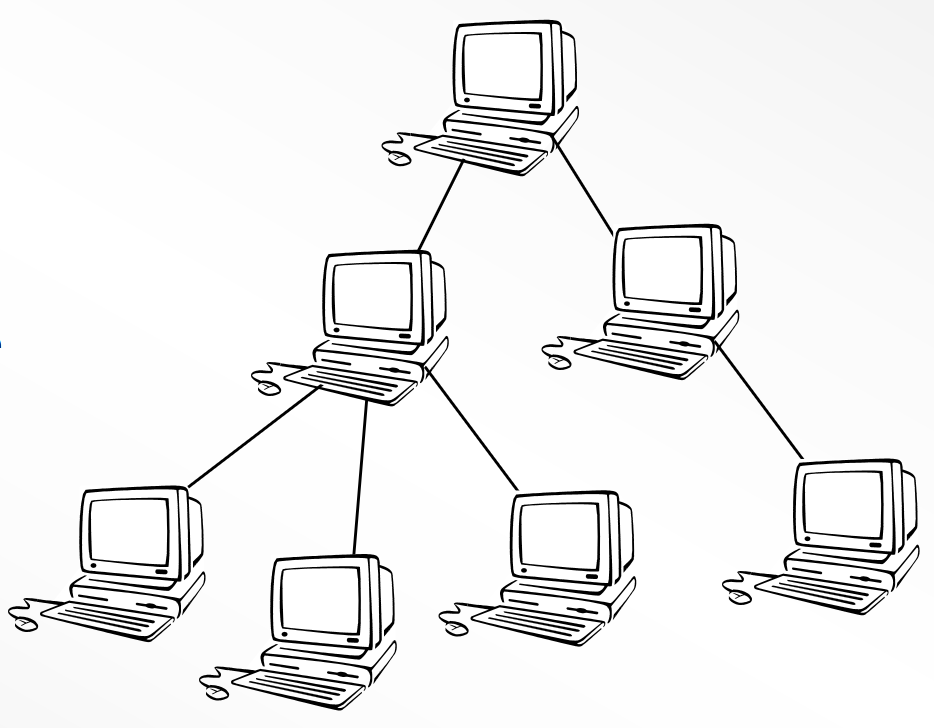
\includegraphics[width=0.3\textwidth]{topologie_arbre.png}
                \caption{Topologie en arbre}
                \label{fig:topologie_arbre}
            \end{figure}
            \begin{description}[style=nextline]
                \item[topologie maillée:]
                Un réseau maillé est un réseau dans lequel deux stations peuvent être mises en
                relation par différents chemins.
            \end{description}
            \begin{figure}[ht]
                \centering
                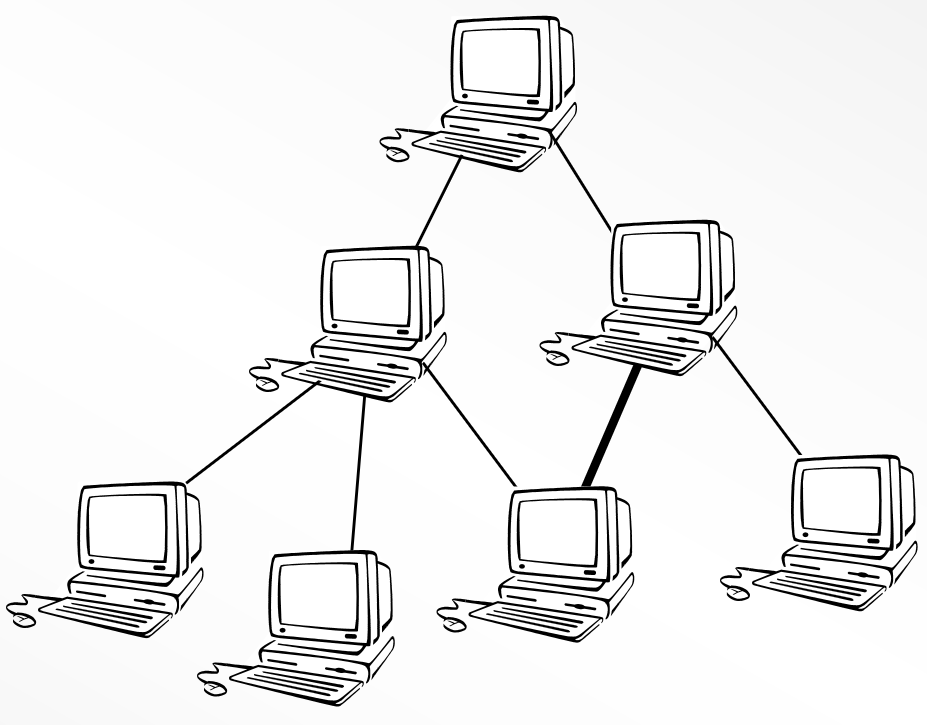
\includegraphics[width=0.3\textwidth]{topologie_maillee.png}
                \caption{Topologie maillée}
                \label{fig:topologie_maillee}
            \end{figure}
        \subsection{taille}
            \begin{description}
                \item[PAN:] personnal area network
                \item[LAN:] local area network
                \item[MAN:] metropolitain area network
                \item[WAN:] wide area network
            \end{description}
            \begin{figure}[ht]
                \centering
                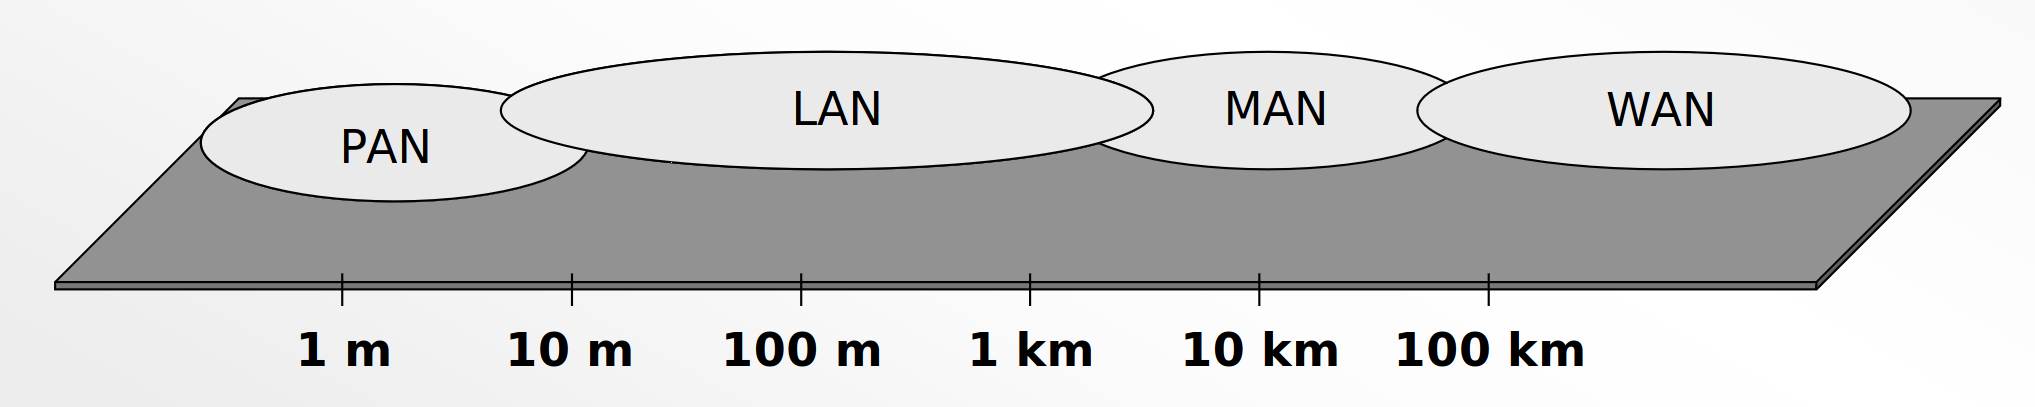
\includegraphics[width=0.8\textwidth]{classification_taille.png}
                \caption{Classification par taille}
                \label{fig:classification_taille}
            \end{figure}
    \section{architectures protocolaires}
        \subsection{modèle OSI}
            \begin{description}
                \item[couches hautes:]Les couches hautes comportent les fonctions de
                traitement sur les données transportées.(5.7)
                \item[couches basses:]Les couches basses garantissent aux couches hautes
                que le transfert d’information se réalise correctement.
                Elles comportent les fonctions de transmission de
                données.(1.4)
            \end{description}
            7: application\\
            6: présentation\\
            5: session\\
            4: transport\\
            3: réseau\\
            2: liaison\\
            1: physique\\
        \subsection{modèle TCP/IP}
            Le modèle est similèrement le même sauf qu'il possède moins de couche que le modèle précédent.\\
            4: application (5.7)\\
            3: transport (4)\\
            2: réseau (3)\\
            1: accès au réseau (1.2)\\
        \subsection{autre}
            Les machines de système relais ne vont utiliser au maximum que les trois premières couches (physique/liaison/réseau).
            Car elles n'ont pas besoin de connaître le message qui se trouve à l'intérieur pour transmettre au destinataire.
    \section{bases théoriques de la transmission des données}
        \subsection{transmision des données}
            L’impulsion électrique représentative d’un élément binaire est affaiblie et
            déformée par le système de transmission.\\
            Ces déformations dépendent du spectre du signal (la nature de celui-ci), ou de la bande passante (la réponse en fréquence du système).\\
            La période \(T\) est définie comme :
            \[T = \frac{1}{f}\] avec \(f\) la fréquence.
        \subsection{spectre de fréquence}
            Un signal périodique quelconque peut donc être considéré comme une infinité de signaux sinusoïdaux.\\
            Chaque composante peut être représentée par l’énergie ou la puissance qu’elle contient. On obtient ainsi le spectre du signal.\\
            L’espace de fréquence occupé par le spectre se nomme largeur de bande. En théorie, la largeur de bande d’un signal non sinusoïdal est infinie.
        \subsection{bande passante}
            Un système de transmission ne transmet pas toutes les fréquences. La courbe de réponse en fréquence d’un système peut être obtenu en utilisant 
            un générateur dont on fait varier la fréquence à tension constante.\\
            le signal en sortie du système n’est plus l’image de celui en entrée. On dit qu’il y a distorsion.\\
            On appelle bande passante à n décibels (dB) l’espace de fréquences tel que tout signal appartenant à cet intervalle ne subisse, au plus, 
            qu’un affaiblissement de n dB : atténuation (dB) = 10 x log10(puissance reçue / puissance transmise).\\
            La largeur de bande d’un signal correspond à la bande passante minimale que le système doit posséder pour restituer correctement l’information.
        \subsection{débit et temps de transfert}
        Le terme de bande passante est utilisé pour désigner un espace fréquentiel (Hz), mais aussi pour qualifier le débit binaire d’un système (bit/s).\\
        Le débit binaire mesure la vitesse de transmission des informations sur un canal (en bit/s), c’est-à-dire le nombre de bits pouvant 
        être transmis en une seconde.\\
        Le temps nécessaire pour envoyer un message sur le canal est égal au nombre de bits à émettre, divisé par le débit binaire du canal.\\
        Le temps de propagation est le temps nécessaire au signal pour parcourir le support d’un bout à l’autre de la liaison. Il dépend de la nature 
        du support, de la distance et de la fréquence du signal.\\
        Le temps de transfert est le temps nécessaire pour que le message émis à travers le réseau soit reçu complètement par le destinataire.\\
        temps de transfert = temps de transmission + temps de propagation
            


\end{document}
